\documentclass{acm_proc_article-sp}
\usepackage{subfiles}

\usepackage[italian]{babel}
\usepackage[utf8]{inputenc}
\usepackage{url}

\begin{document}

\title{Reminiscens, una knowledge base di risorse storiche per supportare la reminiscenza}
\subtitle{[Extended Abstract]
\titlenote{A full version of this paper is available as
\textit{Author's Guide to Preparing ACM SIG Proceedings Using
\LaTeX$2_\epsilon$\ and BibTeX} at
\texttt{www.acm.org/eaddress.htm}}}
 

\numberofauthors{5} %  in this sample file, there are a *total*
% of EIGHT authors. SIX appear on the 'first-page' (for formatting
% reasons) and the remaining two appear in the \additionalauthors section.
%
\author{
% 1st. author
\alignauthor
Nicola Parrello\\
       \affaddr{Università degli studi di Trento}\\
       \affaddr{1932 Wallamaloo Lane}\\
       \affaddr{Wallamaloo, New Zealand}\\
       \email{parrello.nicola@gmail.com}
% 2nd. author
\alignauthor
Wally Will\titlenote{The secretary disavows
any knowledge of this author's actions.}\\
       \affaddr{Institute for Clarity in Documentation}\\
       \affaddr{P.O. Box 1212}\\
       \affaddr{Dublin, Ohio 43017-6221}\\
       \email{webmaster@marysville-ohio.com}
% 3rd. author
\alignauthor
Carmen Sandiego\titlenote{This author is the
one who did all the really hard work.}\\
       \affaddr{The Th{\o}rv{\"a}ld Group}\\
       \affaddr{1 Th{\o}rv{\"a}ld Circle}\\
       \affaddr{Hekla, Iceland}\\
       \email{larst@affiliation.org}
}
% There's nothing stopping you putting the seventh, eighth, etc.
% author on the opening page (as the 'third row') but we ask,
% for aesthetic reasons that you place these 'additional authors'
% in the \additional authors block, viz.
\additionalauthors{Additional authors: John Smith (The Th{\o}rv{\"a}ld Group,
email: {\texttt{jsmith@affiliation.org}}) and Julius P.~Kumquat
(The Kumquat Consortium, email: {\texttt{jpkumquat@consortium.net}}).}
\date{30 July 1999}
% Just remember to make sure that the TOTAL number of authors
% is the number that will appear on the first page PLUS the
% number that will appear in the \additionalauthors section.

\maketitle
\subfile{abstract}

% A category with the (minimum) three required fields
\category{H.4}{Information Systems Applications}{Miscellaneous}
%A category including the fourth, optional field follows...
\category{D.2.8}{Software Engineering}{Metrics}[complexity measures, performance measures]

\terms{Theory}

\keywords{ACM proceedings, \LaTeX, text tagging} % NOT required for Proceedings

\subfile{intro}

\begin{figure*}[t]
\centering
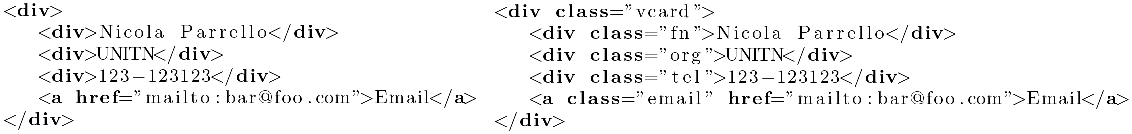
\includegraphics[width=1.0\textwidth]{microformats.pdf}
\caption{Un contatto senza e con il microformato hCard}
\label{fig:microformats}
\end{figure*}

\subfile{sota}

\subfile{problem}

\begin{figure*}[t]
\centering
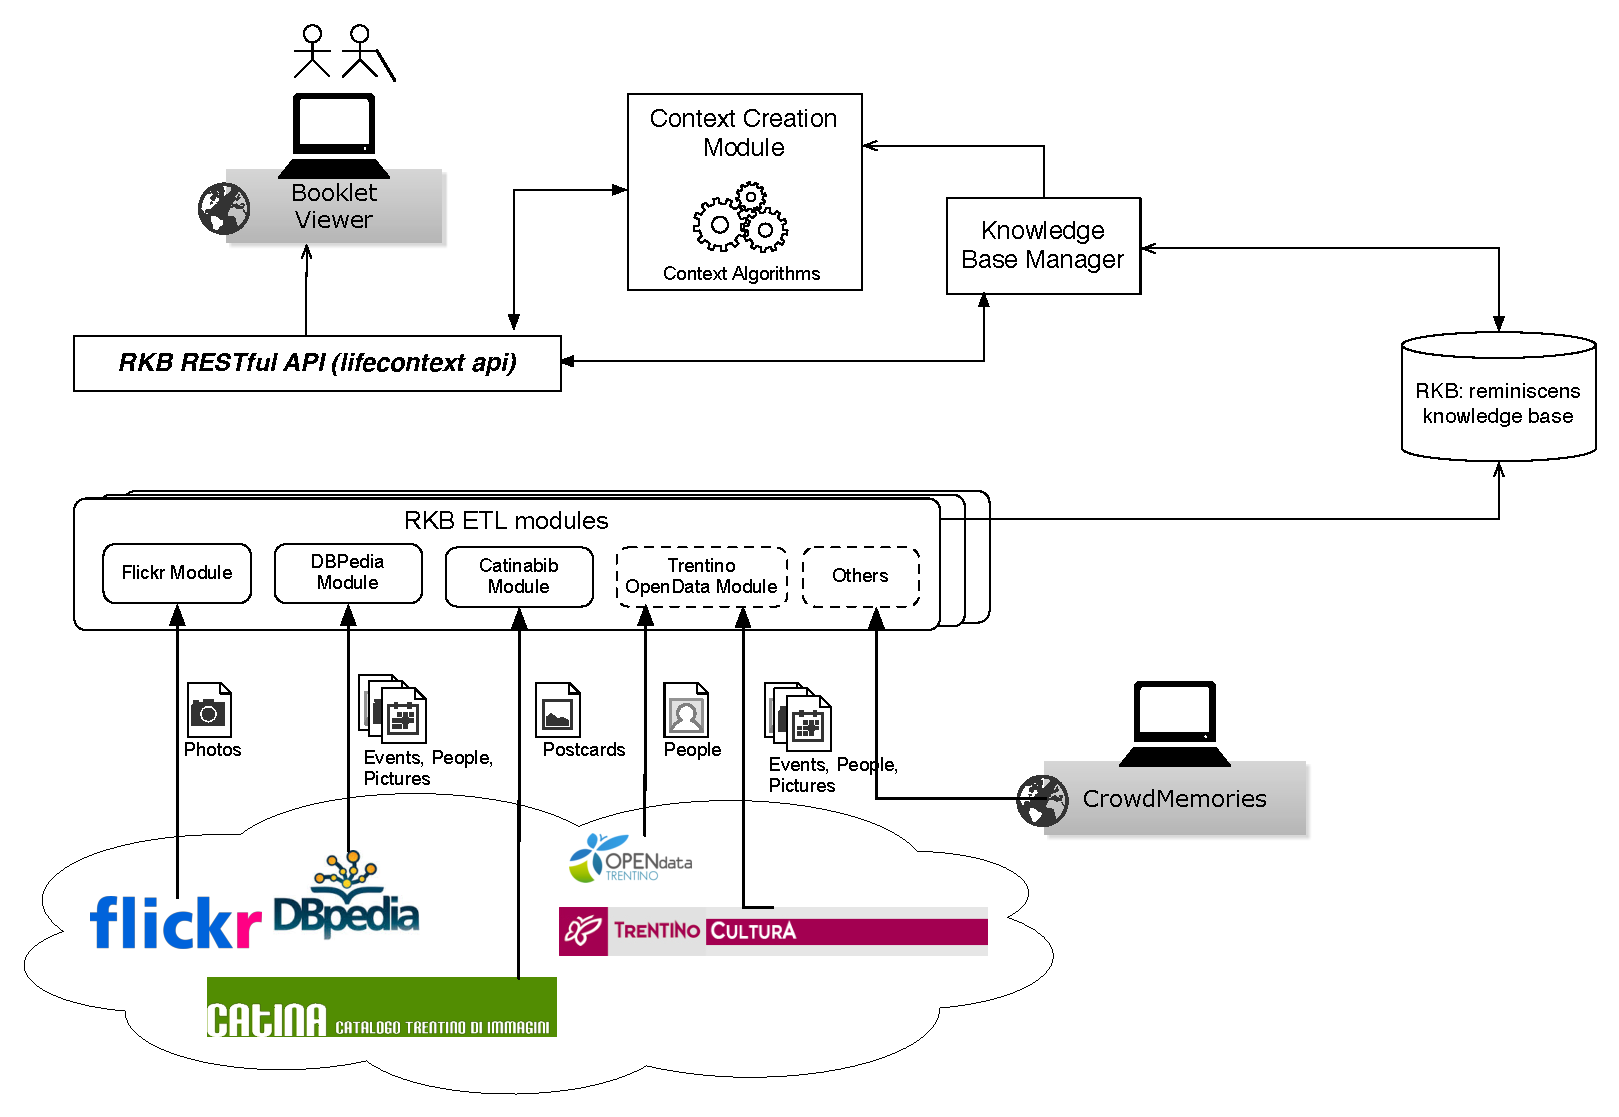
\includegraphics[width=1.0\textwidth]{architecture.pdf}
\caption{Architettura di Reminiscens}
\end{figure*}

\subfile{solution}

\begin{table}
\parbox{.45\linewidth}{
\centering
\begin{tabular}{|r|l|}
\hline
Tipo & Numero \\
\hline
Immagini & 548 \\
Canzoni & 1587 \\
Eventi & 630 \\
Persone famose & 479 \\
\hline
\end{tabular}
\caption{Tipi raccolti}
\label{tab:entitykind}
}
\hfill
\parbox{.45\linewidth}{
\centering
\begin{tabular}{|r|l|}
\hline
Sorgente & Numero \\
\hline
Flickr & 340 \\
DBpedia & 1168 \\
Catinabib & 208 \\
OpenData Trentino & 463 \\
Crowd e altro & 1065 \\
\hline
\end{tabular}
\caption{Distribuzione delle sorgenti}
\label{tab:entitysource}
}
\end{table}

\subfile{related}

\subfile{conclusions}
%\end{document}  % This is where a 'short' article might terminate

%ACKNOWLEDGMENTS are optional
\section{Acknowledgments}
This section is optional; it is a location for you
to acknowledge grants, funding, editing assistance and
what have you.  In the present case, for example, the
authors would like to thank Gerald Murray of ACM for
his help in codifying this \textit{Author's Guide}
and the \textbf{.cls} and \textbf{.tex} files that it describes.

%
% The following two commands are all you need in the
% initial runs of your .tex file to
% produce the bibliography for the citations in your paper.
\bibliographystyle{abbrv}
\bibliography{sigproc}  % sigproc.bib is the name of the Bibliography in this case
% You must have a proper ".bib" file
%  and remember to run:
% latex bibtex latex latex
% to resolve all references
%
% ACM needs 'a single self-contained file'!
%
%APPENDICES are optional
%\balancecolumns
\appendix
%Appendix A
\section{Il Booklet come applicazione per il testing}
Nella sezione dedicata alla soluzione è stato presentato brevemente il Booklet, un’interfaccia pensata per svolgere una delle funzioni di base di Reminiscens, cioè quella di mostrare contenuti che possano risultare familiari all’utente in modo da stimolare l’afflusso di ricordi e far partire la narrazione di episodi correlati al contenuto presentato. Tale applicazione è stata intesa per permettere, come sviluppo futuro, alle famiglie degli anziani la personalizzazione del booklet, aggiungendo ad esempio immagini e musica di propria scelta; il tutto per riuscire a creare un “aggregatore di ricordi” che sia il più efficace possibile. Come anticipato a [\ref{subsubsec:booklet}], la scelta da noi compiuta è quella di offrire un’interfaccia che riprende un libro antico, con una grossa copertina in pelle e il titolo dorato, il tutto con uno sfondo che rappresenta la superficie in legno massiccio di un vecchio tavolo, in modo da mostrare un ambiente familiare che possa essere il primo passo per andare oltre il gap che indubbiamente esiste tra gli anziani e le nuove tecnologie; proprio per come è stata pensata, la UI si presta perfettamente ad un’attività preliminare di testing. Per verificare la bontà delle scelte di design, così come l’adeguatezza di alcuni dati raccolti dai moduli ETL, si potrebbe pensare a un workshop avvalendosi della collaborazione di un centro ricreativo per anziani, strutturato in questo modo: dopo aver diviso i collaboratori in (4?) gruppi, a ogni gruppo verrebbe assegnato un iPad, con a bordo una versione del booklet con contenuti diversi; l’idea è quella di comporre ogni piattaforma di test con contenuti riguardanti un diverso periodo della vita, tenendo conto delle diverse età dei partecipanti e ottenendo quindi infanzia, giovinezza, età adulta e presente. Ultimo parametro da considerare nella divisione dei gruppi e nella composizione dei booklet è quello del luogo in cui centrare il calcolo del contesto da presentare ai volontari: perchè il workshop possa restituire dei risultati utili, c’è bisogno che ognuno possa vedere immagini, ascoltare musica e ricordare eventi che almeno in teoria possano essere significative (e.g. una persona cresciuta a Roma difficilmente potrà rievocare memorie passate guardando delle fotografie del Monte Bondone). Il feedback ricevuto da questa e altre prove è indispensabile per capire se la strada che stiamo percorrendo con Reminiscens è quella giusta e, in caso di difetti del nostro approccio, fornirebbe importanti linee guida per correggerlo.
\subsection{Introduction}
\subsection{The Body of the Paper}
\subsubsection{Type Changes and  Special Characters}
\subsubsection{Math Equations}
\paragraph{Inline (In-text) Equations}
\paragraph{Display Equations}
\subsubsection{Citations}
\subsubsection{Tables}
\subsubsection{Figures}
\subsubsection{Theorem-like Constructs}
\subsubsection*{A Caveat for the \TeX\ Expert}
\subsection{Conclusions}
\subsection{Acknowledgments}
\subsection{Additional Authors}
This section is inserted by \LaTeX; you do not insert it.
You just add the names and information in the
\texttt{{\char'134}additionalauthors} command at the start
of the document.
\subsection{References}
Generated by bibtex from your ~.bib file.  Run latex,
then bibtex, then latex twice (to resolve references)
to create the ~.bbl file.  Insert that ~.bbl file into
the .tex source file and comment out
the command \texttt{{\char'134}thebibliography}.
% This next section command marks the start of
% Appendix B, and does not continue the present hierarchy
\section{More Help for the Hardy}
The acm\_proc\_article-sp document class file itself is chock-full of succinct
and helpful comments.  If you consider yourself a moderately
experienced to expert user of \LaTeX, you may find reading
it useful but please remember not to change it.
\balancecolumns
% That's all folks!
\end{document}
